\documentclass[12pt,a4paper,openright,parskip,final,twoside,en]{csee_msc_thesis} % English, twosided

%%==================================================================
%% PACKAGES
%%==================================================================

\usepackage[T1]{fontenc}
\usepackage{fancybox}
\usepackage{verbatim}
\usepackage{multirow}
\usepackage{xcolor}
\usepackage{parskip}
\usepackage{amsmath}
\usepackage{url}
\usepackage{tikz}
\usepackage{pgfplots}
\usepackage{float}
\usepackage{amssymb}
\usepackage{csquotes}
\usepackage{listings}
\usepackage{parcolumns}

\definecolor{mymauve}{rgb}{0.58,0,0.82}
\definecolor{dkgreen}{rgb}{0,0.6,0}
\lstdefinelanguage
[mips]{Assembler}
{
    morekeywords={loop},
    keywordstyle=\color{mymauve},
    classoffset=1,
    morekeywords={
        lw,add,addi,sw,lw,bge
    },
    keywordstyle=\color{blue},
    classoffset=0,
    morecomment=[l][\color{dkgreen}]{\#},
}

\usepackage{caption,subcaption} % for tables and figures
\usepgfplotslibrary{groupplots}
\usetikzlibrary{matrix,positioning}

\pgfplotsset{compat=1.11}

\usetikzlibrary{positioning,calc,fit}

\definecolor{mybluei}{RGB}{124,156,205}
\definecolor{myblueii}{RGB}{73,121,193}
\definecolor{mygreen}{RGB}{202,217,126}
\definecolor{mydarkgreen}{RGB}{38,175,0}
\definecolor{myred}{RGB}{255,23,23}
\definecolor{mypink}{RGB}{233,198,235}
\definecolor{mygrey}{RGB}{191,193,192}
\definecolor{myyellow}{RGB}{215,226,0}

\lstset{
    commentstyle=\color{green},
    keywordstyle=\color{blue},
    morecomment=[l]{;}
}

% this length is used to control the width of the light blue frame
% for the upper part of the diagram
\newlength\myframesep
\setlength\myframesep{8pt}

\pgfdeclarelayer{background}
\pgfsetlayers{background,main}

\pgfkeys{
    /tikz/node distance/.append code={
        \pgfkeyssetvalue{/tikz/node distance value}{#1}
    }
}

\newcommand\widernode[5][blueb]{
    \node[
        #1,
        inner sep=0pt,
        shift=($(#2.south)-(#2.north)$),
        yshift=-\pgfkeysvalueof{/tikz/node distance value},
        fit={(#2) (#3)},
    label=center:{\sffamily\bfseries\color{white}#4}] (#5) {};
}

\newcommand{\hilight}[1]{\colorbox{yellow}{#1}}

% DEBUG
\sloppy

\loadglsentries{glossaries}

\begin{document}

%%==================================================================
%% VARIABLES
%%==================================================================
\def\thesistitle{\Large Comparing Android Runtime with native:\\ Fast Fourier Transform on Android}
\def\theauthor{\large André Danielsson}
\def\theaddress{
    KTH -- Royal Institute of Technology\\
    \vspace{3mm}
    Master's Thesis in Computer Science\\
    \vspace{3cm}
    KTH Supervisor: Erik Isaksson\\
    \vspace{5mm}
    Bontouch Supervisor: Erik Westenius\\
    \vspace{5mm}
    Examiner: Olle Bälter
}
\def\theabstract{This thesis investigates the performance differences between Java code compiled by Android Runtime and C++ code by Clang. For testing the differences, the Fast Fourier Transform (FFT) algorithm was chosen to demonstrate examples of when it is relevant to have high performance computing on a mobile device. Different aspects that could affect the execution time of a program were examined. One test measured the overhead related to the Java Native Interface (JNI) was tested. The results showed that the overhead was insignificant for FFT sizes larger than 64. Another test compared equivalent implementations between Java and native code. The conclusion of this test was that, of the converted algorithms, the Columbia Iterative FFT performed the best in both Java and C++. Vectorization proved to be an efficient optimization alternative for native development. Finally, tests examining the effect of using single-point precision (\texttt{float}) versus double-point precision (\texttt{double}) data types were covered. Choosing \texttt{float} could improve performance as a result of efficient use of cache.

\textbf{Keywords:} \emph{Keyword 1, Keyword 2, Keyword 3, Keyword 4, Keyword 5, Keyword 6, Keyword 7, }
}
\def\thedate{\today}
\def\thepreface{\input{Preface/preface.tex}}
\def\thesweabstract{I denna studie undersöks prestandaskillnaderna mellan Java-kod kompilerad av Android Runtime och C++-kod kompilerad av Clang. För experimenten som mätte skillnaderna användes en Fast Fourier Transform (FFT) för att understryka vilka användningsområden som kräven hög prestanda på en \hl{mobil enhet / mobilenhet / smart telefon / smartphone}. Olika påverkande aspekter vid användningen av en FFT undersöktes. Ett test undersökte hur mycket påverkan Java Native Interface (JNI) hade på ett program i helhet. Resultaten från dessa tester visade att påverkan var mycket liten för FFT-storlekar större än 64. Ett annat test undersökte prestandaskillnader mellan program översatta från Java till C++. Slutsatsen kring dessa tester var att av de översatta algoritmerna var Columbia Iterative FFT den som presterade bäst, både i Java och i C++. \hl{Vektorisering} visade sig vara en effektiv optimiseringsteknik för maskinkodskompilerad kod skriven i C++. Slutligen utfördes tester som undersökte prestandaskillnader mellan flyttalsprecision för datatyperna \texttt{float} och \texttt{double}. \texttt{float} kunde förbättra prestandan genom att på ett effektitvt sätt utnyttja processorns cache.
}

%%==================================================================
%% PREAMBLES
%%==================================================================
\startpreamble
  {\thesistitle}
  {\theauthor}
  {\thedate}
  {\theabstract}
  {\thepreface}
  {\theaddress}
  {\thesweabstract}

%%==================================================================
%% REPORT
%%==================================================================
\makechapter{Introduction}{Introduction\label{ch:introduction}}
\textit{This thesis explores differences in performance between bytecode and natively compiled code. The Fast Fourier Transform algorithm is the main focus of this degree project. Experiments were carried out to investigate how and when it is necessary to implement the Fast Fourier Transform in Java or in C++ on Android.}

%%==================================================================
%% BACKGROUND
%%==================================================================
\section{Background}
Android is an operating system for smartphones and as of November 2016 it is the most used \cite{android:os:popularity}. One reason for this is because it was designed to be run on multiple different architectures \cite{android:os:devices}. Google states that they want to ensure that manufacturers and developers have an open platform to use and therefore releases Android as Open Source software \cite{android:os:opensource}. The Android kernel is based on the Linux kernel although with some alterations to support the hardware of mobile devices.

\gls{android} applications are mainly written in Java to ensure portability in form of architecture independence. By using a virtual machine to run a Java app, you can use the same bytecode on multiple platforms. To ensure efficiency on low resources devices, a virtual machine called Dalvik was developed. Applications (apps) on Android have been run on the Dalvik Virtual Machine (\gls{dvm}) up until Android version 5 \cite{android:dalvik} in November of 2014 \cite{android:dalvik:release}. Since then, Dalvik has been replaced by Android Runtime. Android Runtime, ART for short, differs from Dalvik in that it uses Ahead-Of-Time (\gls{aot}) compilation. This means that the bytecode is compiled during the installation of the app. Dalvik, however, exclusively uses a concept called Just-In-Time (\gls{jit}) compilation, meaning that code is compiled during runtime when needed. ART uses Dalvik bytecode to compile an application, allowing most apps that are aimed at DVM to work on devices running \gls{art}.

To allow developers to reuse libraries written in C or C++ or to write low level code, a tool called Native Development Kit (\gls{ndk}) was released. It was first released in June 2009 \cite{Lin2011} and has since gotten improvements such as new build tools, compiler versions and support for additional Application Binary Interfaces (\gls{abi}). ABIs are mechanisms that are used to allow binaries to communicate using specified rules. With the \gls{ndk}, developers can choose to write parts of an app in so called \emph{native code}. This is used when wanting to do compression, graphics and other performance heavy tasks.


%%==================================================================
%% PROBLEM
%%==================================================================
\section{Problem}
Nowadays, mobile phones are fast enough to handle heavy calculations on the devices themselves. To ensure that resources are spent in an efficient manner, this study has investigated how significant the performance boost is when compiling the Fast Fourier Transform (\gls{fft}) using the \gls{ndk} tools instead of using \gls{art}. Multiple implementations of FFTs were evaluated as well as the effects of the Java Native Interface (\gls{jni}), a framework for communicating between Java code and native static libraries. The following research question was formed on the basis of these topics:

\begin{center}
    \textit{Is there a significant performance difference between implementations of a Fast Fourier Transform (FFT) in native code, compiled by Clang, and Dalvik bytecode, compiled by Android Runtime, on Android?}
\end{center}

%%==================================================================
%% PURPOSE
%%==================================================================
\section{Purpose}
This thesis is a study that evaluates when and where there will be a gain in writing a part of an Android application in C++. One purpose of this study is to educate the reader about the cost, in performance and effort, of porting parts of an app to native code using the Native Development Kit (\gls{ndk}). Another is to explore the topic of performance differences between Android Runtime (\gls{art}) and native code compiled by Clang/\gls{llvm}. Because \gls{art} is relatively new (Nov 2014) \cite{android:dalvik:release}, this study would contribute with more information about to the performance of \gls{art} and how compares to native code compiled by the \gls{ndk}. The results of the study can also be used to value the decision of implementing a given algorithm in native code instead of Java. It is valuable to know how efficient an implementation in native code is, depending on the size of the data.
% it performs compared to 

The reason you would want to write a part of an application in native code is to potentially get better execution times on computational heavy tasks such as the Fast Fourier Transform (\gls{fft}). The \gls{fft} is an algorithm that computes the Discrete Fourier Transform (\gls{dft}) of a signal. It is primarily used to analyze the components of a signal. This algorithm is used in signal processing and has multiple purposes such as image compression (taking photos), voice recognition (Siri, Google Assistant), fingerprint scanning (unlocking device). Example apps could be a step counter that analyzes the accelerometer data or a music recognizer that uses the microphone to record sound. Another reason you would want to write native libraries is to reuse already written code in C or C++ and incorporate it into your project. This allows app functionality to become platform independent. Component code can then be shared with a computer program and an iOS app.

% MAYBE NOT RELEVANT?
% Some of the findings in this thesis can help decide which method of programming for Android that should be used for a given problem. For some problems, it is necessary to choose the appropriate programming method to ensure that an application is smooth and responsive. It is therefore important to know when and where it is necessary to optimize code. Further, when developing for Android there are multiple types of problems that occur and it is relevant to know which problems are worth solving in \gls{ndk} rather than the Software Development Kit (\gls{sdk}).

%%==================================================================
%% GOAL
%%==================================================================
\section{Goal}
The goal of this project was to examine the efficiency of ART and how it compares to natively written code using the \gls{ndk} in combination with the Java Native Interface (\gls{jni}). This report presents a study that investigates the relevance of using the \gls{ndk} to produce efficient code. Further, the cost to pass through the \gls{jni} is also a factor when analysing the code. A discussion about to what extent the efficiency of a program has an impact on the simplicity of the code is also present. For people who are interested to know about the impacts of implementing algorithms in C++ for Android, this study could be of some use.

%%==================================================================
%% METHOD
%%==================================================================
\section{Procedure}
%% KEYWORDS
%% NDK, Android, Benchmark*, Java, C, C++, Dalvik, Runtime, ART, efficien*, JNI,
%% FFT, Fast Fourier Transform, Fourier Transform, 

The method used to find the relevant literature and previous studies was to search through databases using boolean expressions. By specifying synonyms and required keywords, additional literature could be found. Figure~\ref{fig:db:search} contains an expression that was used to narrow down the search results to relevant articles.

\ifrelease
\begin{figure}[H]
    \centering
    \begin{align*}
        (\text{NDK OR JNI})               & \text{ AND } \\
        \text{Android}                    & \text{ AND } \\
        (\text{benchmark* OR efficien*})  & \text{ AND } \\
        (\text{Java OR C OR C++})         & \text{ AND } \\
        (\text{Dalvik OR Runtime OR ART}) &
    \end{align*}
    \caption{Expression used to filter out relevant articles}
    \label{fig:db:search}
\end{figure}
\fi

This is a strictly quantitative study, meaning numerical data and its statistical significance was the basis for the discussion. The execution time of the programs varied because of factors such as scheduling, CPU clock frequency scaling and other uncontrollable behaviour caused by the operating system. To get accurate measurements, a mean of a large numbers of runs were calculated for each program. Additionally, it was also necessary to calculate the standard error of each set of execution times. With the standard error we can determine if the difference in execution time between two programs are statistically significant or not.

Four different tests were carried out to gather enough data to be able to make reasonable statements about the results. The first one was to find out how significant the overhead of \gls{jni} is. This is important to know to be able to see exactly how large the cost of going between Java and native code is in relation to the actual work. The second test was a comparison between multiple well known libraries to find how much they differ in performance. In the third test, two comparable optimized implementations of \gls{fft}s were chosen, one recursive and one iterative in C++. These implementations were optimized using NEON, a vectorization library for the ARM architecture. In the fourth and final test, the \texttt{float} and \texttt{double} data types were compared.


%%==================================================================
%% DELIMITATIONS
%%==================================================================
\section{Delimitations}
This thesis does only cover a performance evaluation of the \gls{fft} algorithm and does not go into detail on other related algorithms. The decision of choosing the \gls{fft} was due to it being a common algorithm to use in digital signal analysis which is useful in many mobile applications. This thesis does not investigate the performance differences for \gls{fft} in parallel due to the complexity of the Linux kernel used on Android. This would require more knowledge outside the scope of this project and would result in this thesis being too broad. The number of optimization methods covered in this thesis were also delimited to the scope of this degree project.

\section{Limitations}
The tests were carried out on the same phone under the same circumstances to reduce the number of affecting factors. By developing a benchmark program that run the tests during a single session, it was possible to reduce the varying factors that could affect the results. Because you cannot control the Garbage Collector in Java, it is important to have this in mind when constructing tests and analyzing the data.

%%==================================================================
%% ETHICS AND SUSTAINABILITY
%%==================================================================
\section{Ethics and Sustainability}
An ethical aspect of this thesis is that because there could be people making decisions based on this report, it is important that the conclusions are presented together with its conditions so that there are no misunderstandings. Another important thing is that every detail of each test is explicitly stated so that every test can be recreated by someone else. Finally, it is necessary to be critical of the results and find how reasonable the results are.

Environmental sustainability is kept in mind in this investigation because there is an aspect of battery usage in different implementations of algorithms. The less number of instructions an algorithm require, the faster will the CPU lower its frequency, saving power. This will also have an influence on the user experience and can therefore have an impact on the society aspect of sustainability. If this study is used as a basis on a decision that have an economical impact, this thesis would fulfil the economical sustainability goal.

%%==================================================================
%% OUTLINE
%%==================================================================
\section{Outline}
\begin{itemize}
    \item \textit{\textbf{Chapter~\ref{ch:introduction} - Introduction --}} Introduces the reader to the project. This chapter describes why this investigation is beneficial in its field and for whom it is useful.
    \item \textit{\textbf{Chapter~\ref{ch:background} - Background --}} Provides the reader with the necessary information to understand the content of the investigation.
    \item \textit{\textbf{Chapter~\ref{ch:method} - Method --}} Discusses the hardware, software and methods that are the basis of the experiment. Here, the methods of measurement presented and chosen.
    \item \textit{\textbf{Chapter~\ref{ch:results} - Results --}} The results of the experiments are presented here.
    \item \textit{\textbf{Chapter~\ref{ch:discussion} - Discussion --}} Discussion of results and the chosen method.
    \item \textit{\textbf{Chapter~\ref{ch:conclusion} - Conclusion --}} Summary of discussion and future work.
\end{itemize}


\makechapter{Background}{Background\label{ch:background}}
\textit{The process of developing for Android, how an app is installed and how it is being run is explained in this chapter. Additionally, common optimization techniques are described so that we can reason about the results. Lastly, some basic knowledge of the Discrete Fourier Transform is required when discussing differences in FFT implementations. }

\section{Android SDK}
To allow developers to build Android apps, Google developed a Software Development Kit (\gls{sdk}) to facilitate the process of writing Android applications. The Android \gls{sdk} software stack is described in Figure~\ref{fig:sdk}. The Linux kernel is at the base of the stack, handling the core functionality of the device. Detecting hardware interaction, process scheduling and memory allocation are examples of services provided by the kernel. The Hardware Abstraction Layer (\gls{hal}) is an abstraction layer above the device drivers. This allows the developer to interact with hardware independent on the type of device \cite{android:hal}.

The native libraries are low level libraries, written in C or C++, that handle functionality such as the Secure Sockets Layer (\gls{ssl}) and Open GL \cite{komatineni2012pro}. Android Runtime (\gls{art}) features Ahead-Of-Time (\gls{aot}) compilation and Just-In-Time (\gls{jit}) compilation, garbage collection and debugging support \cite{android:sdk:stack}. This is where the Java code is being run and because of the debugging and garbage collection support, it is also beneficial for the developer to write applications against this layer.

The Java \gls{api} Framework is the Java library you use when controlling the Android UI. It is the reusable code for managing activities, implementing data structures and designing the application. The System Application layer represents the functionality that allows a third-party app to communicate with other apps. Example of usable applications are email, calendar and contacts \cite{android:sdk:stack}.

All applications for Android are packaged in so called Android Packages (\gls{apk}). These APKs are zipped archives that contain all the necessary resources required to run the app. Such resources are the AndroidManifest.xml file, Dalvik executables (.dex files), native libraries and other files the application depends on.

\ifrelease
\begin{figure}
    \centering

    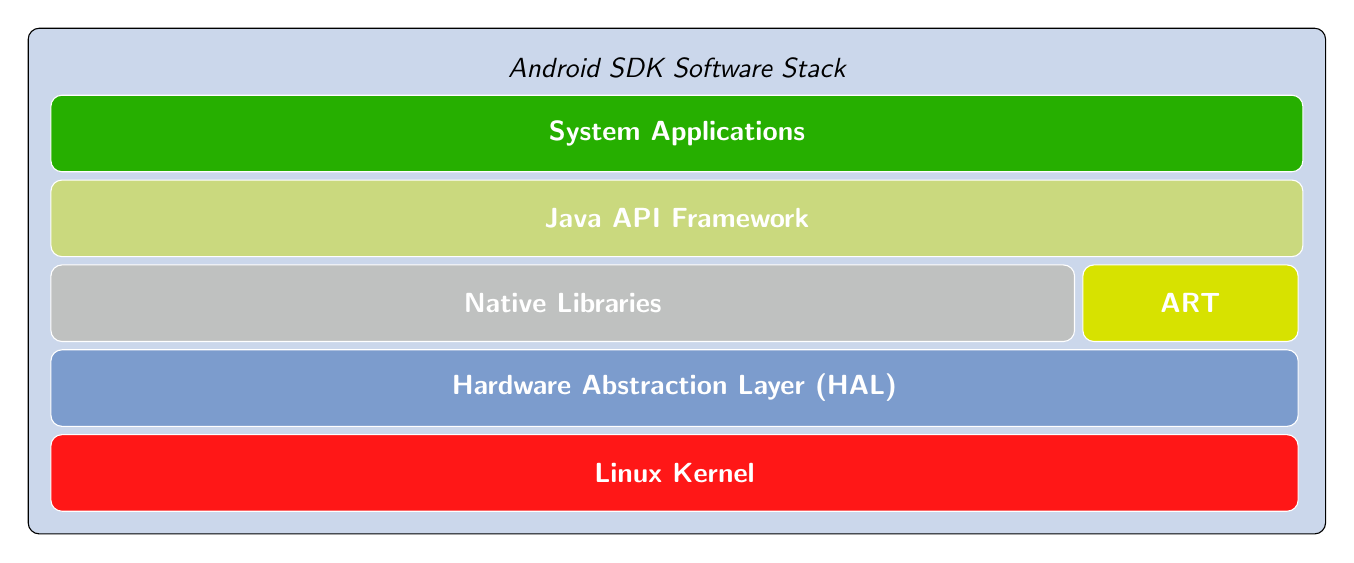
\begin{tikzpicture}[node distance=3pt,outer sep=0pt,
            blueb/.style={
                draw=white,
                fill=mybluei,
                rounded corners,
                text width=2.5cm,
                font={\sffamily\bfseries\color{white}},
                align=center,
                text height=12pt,
            text depth=9pt},
            greenb/.style={blueb,fill=mygreen},
            darkgreenb/.style={blueb,fill=mydarkgreen},
            redb/.style={blueb,fill=myred},
            greyb/.style={blueb,fill=mygrey},
            yellowb/.style={blueb,fill=myyellow},
        ]

        \node[label=center:{\sffamily\bfseries\color{white}System Applications},darkgreenb,minimum width=15.9cm] (SysApps) {};

        \node[label=center:{\sffamily\bfseries\color{white}Java API Framework},greenb,minimum width=15.9cm,below=of SysApps] (JAPI) {};

        \node[label=center:{\sffamily\bfseries\color{white}Native Libraries},greyb,below=of JAPI,minimum width=13cm,xshift=-1.45cm] (Nat) {};
        \node[label=center:{\sffamily\bfseries\color{white}ART},yellowb,right=of Nat] (Art) {};

        \widernode{Nat}{Art}{Hardware Abstraction Layer (HAL)}{Hal}

        \widernode[redb]{Hal}{Hal}{Linux Kernel}{RCP}
        \begin{pgfonlayer}{background}
            \draw[blueb,draw=black,fill=mybluei!40] 
                ([xshift=-\myframesep,yshift=3\myframesep]current bounding box.north west) 
                rectangle 
                ([xshift=\myframesep,yshift=-\myframesep]current bounding box.south east);
        \end{pgfonlayer}
        \node[font=\sffamily\itshape\color{black},above=of SysApps] {Android SDK Software Stack};
    \end{tikzpicture}
    \caption[Android SDK Software Stack]{Android SDK Software Stack \cite{android:sdk:stack}}
    \label{fig:sdk}
\end{figure}
\fi


\section{Dalvik Virtual Machine}
% Why is Dalvik Virtual Machine used?
Compiled Java code is executed on a virtual machine called the Java Virtual Machine (\gls{jvm}). The reason for this is to allow compiled code to become portable. This way, every device, independent on architecture, with a \gls{jvm} installed will be able to run the same code. The Android operating system is designed to be installed on many different devices \cite{android:os:devices}. Because of the many different devices, user applications would have to be compiled for all possible platforms it should work on. For this reason, Java bytecode is a sensible choice when wanting to distribute compiled applications.

The Dalvik Virtual Machine (\gls{dvm}) is the VM initially used on Android. One difference between \gls{dvm} and \gls{jvm} is that the \gls{dvm} uses a register-based architecture while the \gls{jvm} uses a stack-based architecture. The most common virtual machine architecture is the stack-based \cite[p.~158]{craig2010virtual}. A stack-based architecture evaluates each expression directly on the stack and always has the last evaluated value on top of the stack. Thus, only a stack pointer is needed to find the next instruction on the stack.

Contrary to this behaviour, a register-based virtual machine works more like a CPU. It uses a set of registers where it will place operands by fetching them from memory. One advantage of using a register-based architecture is that fetching data between registers is faster than fetching or storing data onto the hardware stack. The biggest disadvantage of using register-based architecture is that the compilers must be more complex than for stack-based architecture. This is because the code generators must take register management into consideration \cite[p.~159-160]{craig2010virtual}.

The \gls{dvm} is a virtual machine optimized for devices where resources are limited \cite{android:dalvik:internals}. The main focus of the \gls{dvm} is to lower memory consumption and lower the number of instructions needed to fulfil a task. Using register-based architecture, it is possible to execute more virtual machine instructions compared to a stack-based architecture \cite{shi2008virtual}. 

% http://www.android-app-developer.co.uk/android-app-development-docs/android-jit-compiler-androids-dalvik-vm.pdf
% https://developer.android.com/about/versions/nougat/android-7.0.html

Dalvik executables, or \gls{dex} files, are the files where Dalvik bytecode is stored. They are created by converting a Java class file to the \gls{dex} format. They are of a different structure than Java class files. Some differences are the header types that describes the data. One example of the differences is the string constant fields that are present in the \gls{dex}-file. % FIND REFERENCE FROM GOOGLE IO ABOUT DALVIK??

\section{Android Runtime}
Android Runtime is the new default runtime for Android as of version 5.0 \cite{android:dalvik}. The big improvement over Dalvik is the fact that applications are compiled to binary when they are installed on the device, rather than during runtime of the app. This results in faster start-up \cite{li2016advanced} and lets the compiler use more heavy optimization that is not otherwise possible during runtime. However, if the whole application is compiled ahead of time it is no longer possible to do any runtime optimizations. An example of a runtime optimization is to inline methods or functions that are called frequently.

When an app is installed on the device, a program called \textbf{dex2oat} converts a \gls{dex}-file to an executable file called an oat-file \cite{android:art:dalvik}. This oat-file is in the Executable and Linkable Format (ELF) and can be seen as a wrapper of multiple \gls{dex}-files \cite{Dresel2016}. An improvement made in Android Runtime is the optimized garbage collector. Changes include a decrease from two to one GC pause, reduced memory fragmentation (reduces calls to \texttt{GC\_FOR\_ALLOC}) and parallelization techniques to lower the time it takes to collect~\cite{android:art:dalvik}. There are two common garbage collects plans, Sticky Concurrent Mark Sweep (Sticky CMS) and Partial Concurrent Mark Sweep (Partial CMS). Sticky CMS does not move data and does only reclaim data that has been allocated since the last garbage collect \cite{android:art:gc}. Partial CMS frees from the active heap of the process \cite[p.~122]{sillars2015high}.

\section{Native Development Kit}
Native Development Kit (\gls{ndk}) is a set of tools to help writing native apps for Android. It contains the necessary libraries, compilers, build tools and debugger for developing low level libraries. Google recommends using the \gls{ndk} for two reasons: run computationally intensive tasks and usage of already written libraries \cite{android:ndk:guides}. Because Java is the supported language on Android, due to security and stability, native development is not recommended to use to build full apps, with an exception when developing games.

Historically, native libraries have been built using Make. Make is a tool used to coordinate compilation of source files. Android makefiles, \texttt{Android.mk} and \texttt{Application.mk}, are used to set compiler flags, choose which architectures that a project should be compiled for, location of source files and more. With Android Studio 2.2 \gls{cmake} was introduced as the default build tool \cite{android:studio:cmake}. CMake is a more advanced tool for generating and running build scripts.

At each compilation, the architectures the source files will be built against must be specified. The source file(s) generated will be placed in a folder structure where the source file is located in a folder that determines the architecture. Each architecture-folder is located in a folder called \texttt{lib}. This folder will be placed at the root of the \gls{apk}.

\begin{verbatim}
lib/
|--armeabi-v7a/
|  |--lib[libname].so
|--x86/
   |--lib[libname].so
\end{verbatim}

\subsection{Java Native Interface}
% GOOD => https://www.fer.unizg.hr/_download/repository/jni.pdf <=
To be able to call native libraries from Java code, a framework named Java Native Interface (\gls{jni}) is used. Using this interface, C/C++ functions are mapped as methods and primitive data types are converted between Java and C/C++. For this to work, special syntax is needed for \gls{jni} to recognize which method in which class a native function should correspond to.

To mark a function as native in Java, a special keyword called \texttt{native} is used to define a method. The library which implements this method must also be included in the same class. By using the \texttt{System.loadLibrary("mylib")} call, we can specify the name of the static library that should be loaded. Inside the native library we must follow a function naming convention to map a method to a function. The rules are that you must start the function name with \texttt{Java} followed by the package, class and method name. Figure~\ref{fig:native} demonstrates how to map a method to a native function.

\ifrelease
\begin{figure}[H]
\begin{center}
    \texttt{private native int myFun();}\\
    $\Updownarrow$
    \begin{verbatim}
      JNIEXPORT jint JNICALL
      Java_com_example_MainActivity_myFun (JNIEnv *env, jobject thisObj)
    \end{verbatim}
\end{center}
\caption{Native method declaration to implementation.}
\label{fig:native}
\end{figure}
\fi

The \gls{jni} also provides a library for C and C++ for handling the special \gls{jni} data types. They can be used to determine the size of a Java array, get position of elements of an array and handling Java objects. In C and C++ you are given a pointer to a list of \gls{jni} functions (\texttt{JNIEnv*}). With this pointer, you can communicate with the JVM \cite[p.~22]{liang1999java}. You typically use the \gls{jni} functions to fetch data from handled by the JVM, call methods and create objects.

The second parameter to a \gls{jni} function is of the \texttt{jobject} type. This is the current Java object that has called this specific \gls{jni} function. It can be seen as an equivalent to the \texttt{this} keyword in Java and C++ \cite[p.~23]{liang1999java}. There is a function-pair available in the \texttt{JNIEnv} pointer called \texttt{GetDoubleArrayElements()} and \texttt{ReleaseDoubleArrayElements()}. There are also functions for other primitive types such as \texttt{GetIntArrayElements()}, \texttt{GetShortArrayElements()} and others. \texttt{GetDoubleArrayElements()} is used to convert a Java array to a native memory buffer \cite[p.~159]{liang1999java}. This call also tries to \enquote{pin} the elements of the array.

\emph{Pinning} allows \gls{jni} to provide the reference to an array directly instead of allocating new memory and copying the whole array. This is used to make the call more efficient although it is not always possible. Some implementations of the virtual machine does not allow this because it requires that the behaviour of the garbage collector must be changed to support this \cite[p.~158]{liang1999java}. There are two other functions, \texttt{GetPrimitiveArrayCritical()} and \texttt{ReleasePrimitiveArrayCritical()}, that can be used to avoid garbage collection in native code. Between these function calls, the native code should not run forever, no calls to any of the \gls{jni} functions are allowed and it is prohibited to block a thread that depends on a VM thread to continue.

\subsection{LLVM and Clang}
\gls{llvm} (Low Level Virtual Machine) is a suite that contains a set of compiler optimizers and backends. It is used as a foundation for compiler frontends and supports many architectures. An example of a frontend tool that uses \gls{llvm} is \gls{clang}. Clang is used compile C, C++ and Objective-C source code \cite{clang:comp}.

Clang is as of March 2016 (\gls{ndk} version 11) \cite{android:ndk:revision}, the only supported compiler in the \gls{ndk}. Google has chosen to focus on supporting the Clang compiler instead of the GNU GCC compiler. This means that there is a bigger chance that a specific architecture used on an Android device is supported in the \gls{ndk}. This also allows Google to focus on developing optimizations for these architectures with only one supported compiler.

\section{Code Optimization}

There are many ways your compiler can optimize your code during compilation. This chapter will first present some general optimization measures taken by the optimizer and will then describe some language specific methods for optimization.

\subsubsection{Loop unrolling}
Loop unrolling is a technique used to optimize loops. By explicitly coding multiple iterations in the body of the loop, it is possible to lower the amount of jump instructions in the produced code. Figure~\ref{fig:c:unroll} demonstrates how unrolling works by decreasing the number of iterations but adding lines in the loop body. The loop unroll executes two iterations of the first code per iteration. It is therefore necessary to update the \texttt{i} variable accordingly. Figure~\ref{fig:assembly:unroll} describes how the change could be represented in assembly language.

\ifrelease
\begin{figure}
    \centering
    \begin{subfigure}{.5\textwidth}
        \centering
        \begin{verbatim}
    for (int i = 0; i < 6; ++i) {
        a[i] = a[i] + b[i];
    }

        \end{verbatim}
        \caption{Normal}
        \label{fig:c:unroll:normal}
    \end{subfigure}%
    \begin{subfigure}{.5\textwidth}
        \centering
        \begin{verbatim}
    for (int i = 0; i < 6; i+=2) {
        a[i] = a[i] + b[i];
        a[i+1] = a[i+1] + b[i+1];
    }
        \end{verbatim}
        \caption{One unroll}
        \label{fig:c:unroll:unroll}
    \end{subfigure}
    \caption{Loop unrolling in C}
    \label{fig:c:unroll}
\end{figure}
\fi

The gain in using loop unrolling is that you \enquote{save} the same amount of jump instructions as the amount of \enquote{hard coded} iterations you add. In theory, it is also possible to optimize even more by changing the offset of \texttt{LOAD WORD} instructions as shown in Figure~\ref{fig:assembly:optimized}. Then you would not need to update the iterator as often.

% https://www.cs.umd.edu/class/fall2001/cmsc411/proj01/proja/why.html
\ifrelease
\begin{figure}
    \centering
    \begin{adjustbox}{minipage=\linewidth,scale=0.8}
        \begin{verbatim}
                $s1 - a[] address | $s4 - value of a[x]
                $s2 - b[] address | $s5 - value of b[x]
                $s3 - i           | $s6 - value 6
        \end{verbatim}
        \begin{subfigure}{.55\textwidth}
            \centering
            \begin{lstlisting}[
                    language={[mips]Assembler},
                    basicstyle=\footnotesize,
                    numbers=left,
                    firstnumber=1,
                    numberfirstline=true
                ]
loop: lw $s4, 0($s1) # Load a[i]
      lw $s5, 0($s2) # Load b[i]
      add $s4, $s4, $s5 # a[i] + b[i]
      sw $s4, 0($s1)
      addi $s1, $s1, 4 # next element
      addi $s2, $s2, 4 # next element
      addi $s3, $s3, 1 # i++
      bge $s3, $s6, loop
                \end{lstlisting}
            \caption{Normal}
            \label{fig:unroll:sub1}
        \end{subfigure}%
        \begin{subfigure}{.3\textwidth}
            \centering
            \begin{lstlisting}[
                    language={[mips]Assembler},
                    basicstyle=\footnotesize,
                    numbers=left,
                    firstnumber=1,
                    numberfirstline=true
                ]
loop: lw $s4, 0($s1)
      lw $s5, 0($s2)
      add $s4, $s4, $s5
      sw $s4, 0($s1)
      addi $s1, $s1, 4
      addi $s2, $s2, 4
      addi $s3, $s3, 1
      lw $s4, 0($s1)
      lw $s5, 0($s2)
      add $s4, $s4, $s5
      sw $s4, 0($s1)
      addi $s1, $s1, 4
      addi $s2, $s2, 4
      addi $s3, $s3, 1
      bge $s3, $s6, loop
                \end{lstlisting}
            \caption{One unroll}
            \label{fig:unroll:sub2}
        \end{subfigure}
    \end{adjustbox}
    \caption{Loop unrolling in assembly}
    \label{fig:assembly:unroll}
\end{figure}
\fi


\subsubsection{Inlining}
Inlining allows the compiler to swap all the calls to an inline function with the content of the function. This removes the need to do all the preparations for a function call such as saving values in registers and preparing parameters and return values. This comes at a cost of a larger program if there are many calls to this function in the code and if the function is large. It is very useful to use inline functions in loops that are run many times. This is an optimization that can be used manually in C and C++ using the \texttt{inline} keyword and can also be optimized by the compiler.

\ifrelease
\begin{figure}[h]
    \centering
    \begin{adjustbox}{minipage=\linewidth,scale=0.8}
        \centering
        \begin{verbatim}
                  $s1 - a[] address | $s4 - value of a[x]
                  $s2 - b[] address | $s5 - value of b[x]
                  $s3 - i           | $s6 - value 6
        \end{verbatim}
        \begin{subfigure}{.55\textwidth}
            \centering
            \begin{lstlisting}[
                    language={[mips]Assembler},
                    basicstyle=\footnotesize,
                    numbers=left,
                    firstnumber=1,
                    numberfirstline=true
                ]
loop: lw $s4, 0($s1)
      lw $s5, 0($s2)
      add $s4, $s4, $s5
      sw $s4, 0($s1)
      addi $s1, $s1, 4
      addi $s2, $s2, 4
      addi $s3, $s3, 1
      lw $s4, 0($s1)
      lw $s5, 0($s2)
      add $s4, $s4, $s5
      sw $s4, 0($s1)
      addi $s1, $s1, 4
      addi $s2, $s2, 4
      addi $s3, $s3, 1
      bge $s3, $s6, loop
                \end{lstlisting}
            \caption{One unroll}
            \label{fig:optimized:sub1}
        \end{subfigure}%
        \begin{subfigure}{.3\textwidth}
            \centering
            \begin{lstlisting}[
                    language={[mips]Assembler},
                    basicstyle=\footnotesize,
                    numbers=left,
                    firstnumber=1,
                    numberfirstline=true
                ]
loop: lw $s4, 0($s1)
      lw $s5, 0($s2)
      add $s4, $s4, $s5
      sw $s4, 0($s1)
      lw $s4, 4($s1)
      lw $s5, 4($s2)
      add $s4, $s4, $s5
      sw $s4, 4($s1)
      addi $s1, $s1, 8
      addi $s2, $s2, 8
      addi $s3, $s3, 2
      bge $s3, $s6, loop
                \end{lstlisting}
            \caption{Optimized unroll}
            \label{fig:optimized:sub2}
        \end{subfigure}
    \end{adjustbox}
    \caption{Optimized loop unrolling in assembly}
    % https://www.cs.umd.edu/class/fall2001/cmsc411/proj01/proja/why.html
    \label{fig:assembly:optimized}
\end{figure}
\fi


\subsubsection{Constant folding}
\emph{Constant folding} is a technique used to reduce the time it takes to evaluate an expression in runtime \cite[p.~329]{muchnick1997advanced}. By finding which variables that already have a value, the compiler can calculate and assign constants in compile time instead of during runtime. This method of analyzing the code to find expressions consisting of variables that are possible to calculate is called \emph{Constant Propagation} as seen in Figure~\ref{fig:constant:propagation}.

\ifrelease
\begin{figure}[h]
    \centering
    \begin{adjustbox}{minipage=\linewidth,scale=1.0}
        \begin{subfigure}{.40\textwidth}
            \centering
            \begin{lstlisting}[
                    language={C},
                    basicstyle=\footnotesize,
                ]
      int x = 10;
      int y = x * 5 + 3;
                \end{lstlisting}
            \caption{Before optimization}
            \label{fig:propagation:sub1}
        \end{subfigure}%
        \begin{subfigure}{.50\textwidth}
            \centering
            \begin{lstlisting}[
                    language={C},
                    basicstyle=\footnotesize,
                ]
              int x = 10;
              int y = 53;
                \end{lstlisting}
            \caption{Constant propagation optimization}
            \label{fig:propagation:sub2}
        \end{subfigure}
    \end{adjustbox}
    \caption{Constant Propagation}
    \label{fig:constant:propagation}
\end{figure}
\fi

\subsubsection{Loop Tiling}
When processing elements in a large array multiple times it is beneficial to utilize as many reads from cache as possible. If the array is larger than the cache, it will kick out earlier elements for the next pass through the array. By processing partitions of the array multiple times before going on to next partition, temporal cache locality can help the program run faster. Temporal locality means that you can find a previously referenced value in the cache if you are trying to access it again. As Figure~\ref{fig:loop:tiling} shows, by introducing a new loop that operate over a small enough partition of the array such that every element is in cache, we will reduce the number of cache misses.

\ifrelease
\begin{figure}[h]
    \begin{adjustbox}{minipage=\linewidth,scale=0.8}
        \begin{subfigure}{.50\textwidth}
            \centering
            \begin{lstlisting}[
                    language={C},
                    basicstyle=\footnotesize,
                ]
    for (i = 0; i < NUM_REPS; ++i) {
        for (j = 0; j < ARR_SIZE; ++j) {
            a[j] = a[j] * 17;
        }
    }
                \end{lstlisting}
            \caption{Before loop tiling}
            \label{fig:tiling:sub1}
        \end{subfigure}%
        \begin{subfigure}{.50\textwidth}
            \centering
            \begin{lstlisting}[
                    language={C},
                    basicstyle=\footnotesize,
                ]
        for (j = 0; j < ARR_SIZE; j += 1024) {
            for (i = 0; i < NUM_REPS; ++i) {
                for (k = j; k < (j + 1024); ++k) {
                    a[k] = a[k] * 17;
                }
            }
        }
                \end{lstlisting}
            \caption{After loop tiling}
            \label{fig:tiling:sub2}
        \end{subfigure}
    \end{adjustbox}
    \caption{Loop Tiling}
    \label{fig:loop:tiling}
\end{figure}
\fi


% http://www.azillionmonkeys.com/qed/optimize.html
% => Optimizing compilers for modern architectures <=

% \subsubsection{Loop fission and loop fusion}
% \emph{Loop Fusion} and \emph{Loop Fission} are two ways of changing how loops are executed. They are the opposites of themselves and are used based on the instructions in the loop. The purpose of \emph{Loop Fission} is to separate a statement or statements from each other and have multiple loops. This increases the loop overhead but can become more efficient if the separated loop has good cache locality. As we see in Figure~\ref{fig:fission:sub1}, we read from two arrays, \texttt{b} and \texttt{c}. We cannot know if they are close to each other in memory which can lead to many cache misses every iteration of the loop. If we split the loop as in Figure~\ref{fig:fission:sub2}, we can utilize memory locality to get more efficient code.
%
% \begin{figure}[h]
%     \centering
%     \begin{subfigure}{.45\textwidth}
%         \centering
%         \begin{lstlisting}[
%                 language={C},
%                 basicstyle=\footnotesize,
%                 numbers=left,
%                 firstnumber=1,
%                 numberfirstline=true
%             ]
% for (i = 0; i < 10; ++i) {
%     a[i] = b[i];
%     b[i] = c[i];
% }
%             \end{lstlisting}
%         \caption{Before split}
%         \label{fig:fission:sub1}
%     \end{subfigure}%
%     \begin{subfigure}{.35\textwidth}
%         \centering
%         \begin{lstlisting}[
%                 language={C},
%                 basicstyle=\footnotesize,
%                 numbers=left,
%                 firstnumber=1,
%                 numberfirstline=true
%             ]
% for (i = 0; i < 10; ++i)
%     a[i] = b[i];
% for (i = 0; i < 10; ++i)
%     b[i] = c[i];
%         \end{lstlisting}
%         \caption{After split}
%         \label{fig:fission:sub2}
%     \end{subfigure}
%     \caption{Loop fission}
%     \label{fig:c:loopfission}
% \end{figure}
%
% On the other hand, \emph{Loop Fusion} merges two loops into one because memory locality is possible in one loop. This removes the overhead of having two loops. Because both assignments require reads from the \texttt{a} array that are close to each other, cache locality is possible. Both of these techniques are commonly used by the optimizer in the compiler.
%
% \begin{figure}[h]
%     \centering
%     \begin{subfigure}{.45\textwidth}
%         \centering
%         \begin{lstlisting}[
%                 language={C},
%                 basicstyle=\footnotesize,
%                 numbers=left,
%                 firstnumber=1,
%                 numberfirstline=true
%             ]
% for (i = 1; i < 10; ++i)
%     a[i] = a[i-1];
% for (i = 1; i < 10; ++i)
%     b[i] = a[i];
%             \end{lstlisting}
%         \caption{Before fusion}
%         \label{fig:fusion:sub1}
%     \end{subfigure}%
%     \begin{subfigure}{.35\textwidth}
%         \centering
%         \begin{lstlisting}[
%                 language={C},
%                 basicstyle=\footnotesize,
%                 numbers=left,
%                 firstnumber=1,
%                 numberfirstline=true
%             ]
% for (i = 1; i < 10; ++i) {
%     a[i] = a[i-1];
%     b[i] = a[i];
% }
%         \end{lstlisting}
%         \caption{After fusion}
%         \label{fig:fusion:sub2}
%     \end{subfigure}
%     \caption{Loop fusion}
%     \label{fig:c:loopfusion}
% \end{figure}

\subsection{Java}
In Java, an array is created during runtime and cannot change its size after it is created. This means that it will always be placed on the heap and the garbage collector will handle the memory it resides on when it is no longer needed. By keeping an array reference in scope and reusing the same array, we can circumvent this behaviour and save some instructions by not needing to ask for more memory from the heap.

% Object allocation pool
% CPU usage during runtime
% Garbage collection
% http://www.cubrid.org/blog/dev-platform/understanding-java-garbage-collection/
% Java Performance: The Definitive Guide
% http://www.gamasutra.com/view/news/128161/A_Low_Level_Curriculum_for_C_and_C.php
% https://lwn.net/Articles/250967/
% Hacker's Delight (2nd Edition)
% https://en.wikibooks.org/wiki/C++_Programming/Optimization
% http://www.slideshare.net/cdman83/performance-optimization-techniques-for-java-code
% http://www.agner.org/optimize/optimizing_cpp.pdf
% http://leto.net/docs/C-optimization.php
% http://www.appperfect.com/support/java-coding-rules/optimization.php
% https://developer.android.com/training/articles/perf-tips.html#UseFinal
% http://blog.takipi.com/garbage-collectors-serial-vs-parallel-vs-cms-vs-the-g1-and-whats-new-in-java-8/
% http://stackoverflow.com/questions/9546392/what-triggers-a-full-garbage-collection-in-java
% https://www.itu.dk/people/sestoft/papers/benchmarking.pdf

\subsection{C++}
C and C++ arrays have predefined sizes and are located on the program stack. This makes the program run faster because it does not need to call malloc or new and ask for more memory on the heap. This require that the programmer knows the required size of the array in advance and is not always possible or memory efficient.

\subsubsection{NEON}
% TODO: Explain what intrinsics are
% http://www.crickettechnology.com/blog/?p=691
% http://wanderingcoder.net/2010/07/19/ought-arm/
% http://wanderingcoder.net/2010/06/02/intro-neon/
Android \gls{ndk} includes a tool called \gls{neon} that contains functions which enables Single Instruction Multiple Data (\gls{simd}). SIMD is an efficient way of executing the same type of operation on multiple operands at the same time. Figure~\ref{fig:simd} describes this concept where instead of operating on one piece of data at the time, a larger set of data that uses the same operation can be processed with one operation.

\gls{neon} provides a set of functions compatible with the ARM architecture. These functions can perform operations on double word and quad word registers. The reason you would want to use SIMD because you can have instructions that loads blocks of multiple values and operates on these blocks.  The process starts by reading the data into larger vector registers, operate on these registers and storing the results as blocks \cite{simd:expl}. This way you will have less instructions than if you loaded one element at a time and operated on only that value.

\gls{simd} has some prerequisites on the data that is being processed. Firstly, the data blocks must line up meaning that you cannot operate between two operands that are not in the same area of the block. Secondly, all the operands of a block must be of the same type.

\ifrelease
\begin{figure}
    \centering
    \begin{subfigure}{.45\textwidth}
        \centering
        \begin{tikzpicture}[
                node distance = 0mm,
                start chain=1 going {below=of \tikzchainprevious.south west}, 
                box/.style = {draw, semithick, minimum size=1cm, every on chain/.style={anchor=north west}, outer sep = 0mm, on chain}
            ]
            \foreach \i in {1,...,4}
            {
                \pgfmathtruncatemacro{\y}{\i - 1};
                \pgfmathtruncatemacro{\lab}{(\i - 4) * -1}
                \node[fill=myeggshell,box] (A\lab) at (0, 1.5*\y) {A$_\lab$};
                \node[fill=mylightgreen,box] (B\lab) at (1.6, 1.5*\y) {B$_\lab$};
                \node[fill=mylightred,box] (C\lab) at (4, 1.5*\y) {C$_\lab$};
                \node[fill=none,right of=A\lab,node distance=0.8cm] (plus\i) {+};
                \node[fill=none,right of=B\lab,node distance=1.15cm] (equals\i) {=};
            };
        \end{tikzpicture}
        \caption{Four separate instructions}
        \label{fig:simd:simd1}
    \end{subfigure}%
    \begin{subfigure}{.35\textwidth}
        \centering
        \begin{tikzpicture}[
                node distance = 0mm,
                start chain=1 going {below=of \tikzchainprevious.south west}, 
                box/.style = {draw, semithick, minimum size=1cm, every on chain/.style={anchor=north west}, outer sep = 0mm, on chain}
            ]
            \foreach \i in {1,...,4}
            {
                \pgfmathtruncatemacro{\y}{\i - 1};
                \pgfmathtruncatemacro{\lab}{(\i - 4) * -1}
                \node[fill=myeggshell,box] (A\lab) at (0, 1*\y) {A$_\lab$};
                \node[fill=mylightgreen,box] (B\lab) at (1.6, 1*\y) {B$_\lab$};
                \node[fill=mylightred,box] (C\lab) at (4, 1*\y) {C$_\lab$};
            };
            \node[fill=none] (plus) at (1.3, 0.95) {+};
            \node[fill=none] (equals) at (3.3, 0.95) {=};
        \end{tikzpicture}
        \caption{One instruction with SIMD}
        \label{fig:simd:simd2}
    \end{subfigure}
    \caption[Single Instruction Multiple Data]{Single Instruction Multiple Data \cite{kernel:simd}}
    \label{fig:simd}
\end{figure}
\fi

\section{Discrete Fourier Transform}\label{ch:dft}
The Discrete Fourier Transform (\gls{dft}) is a method of converting a sampled signal from the time domain to the frequency domain. In other words, the \gls{dft} takes an observed signal and dissects each component that would form the observed signal. Every component of a signal can each be described as a sinusoidal wave with a frequency, amplitude and phase.

If we observe Figure~\ref{fig:dft:ex1}, we can see how a signal in time domain looks like in frequency domain. The function displayed in the time domain consists of three sine components, each with its own amplitude and frequency. What the graph of the frequency domain shows, is the amplitude of each frequency. This can then be used to analyze the input signal.

One important thing to note is that you must sample at twice the frequency you want to analyze. The Nyquist sampling theorem states that \cite{signal:aliasing}:
\begin{center}
    \textit{The sampling frequency should be at least twice the highest frequency contained in the signal.}
\end{center}
In other words, you have to be able to reconstruct the signal given the samples \cite[Ch~3]{smith1997scientist}. If you are given a signal that is constructed of frequencies that are at most 500~Hz, your sample frequency must be at least 1000 samples per second to be able to find the amplitude for each frequency.

\ifrelease
\begin{figure}[h]
    \renewcommand\thesubfigure{(\alph{subfigure})}
    \centering
    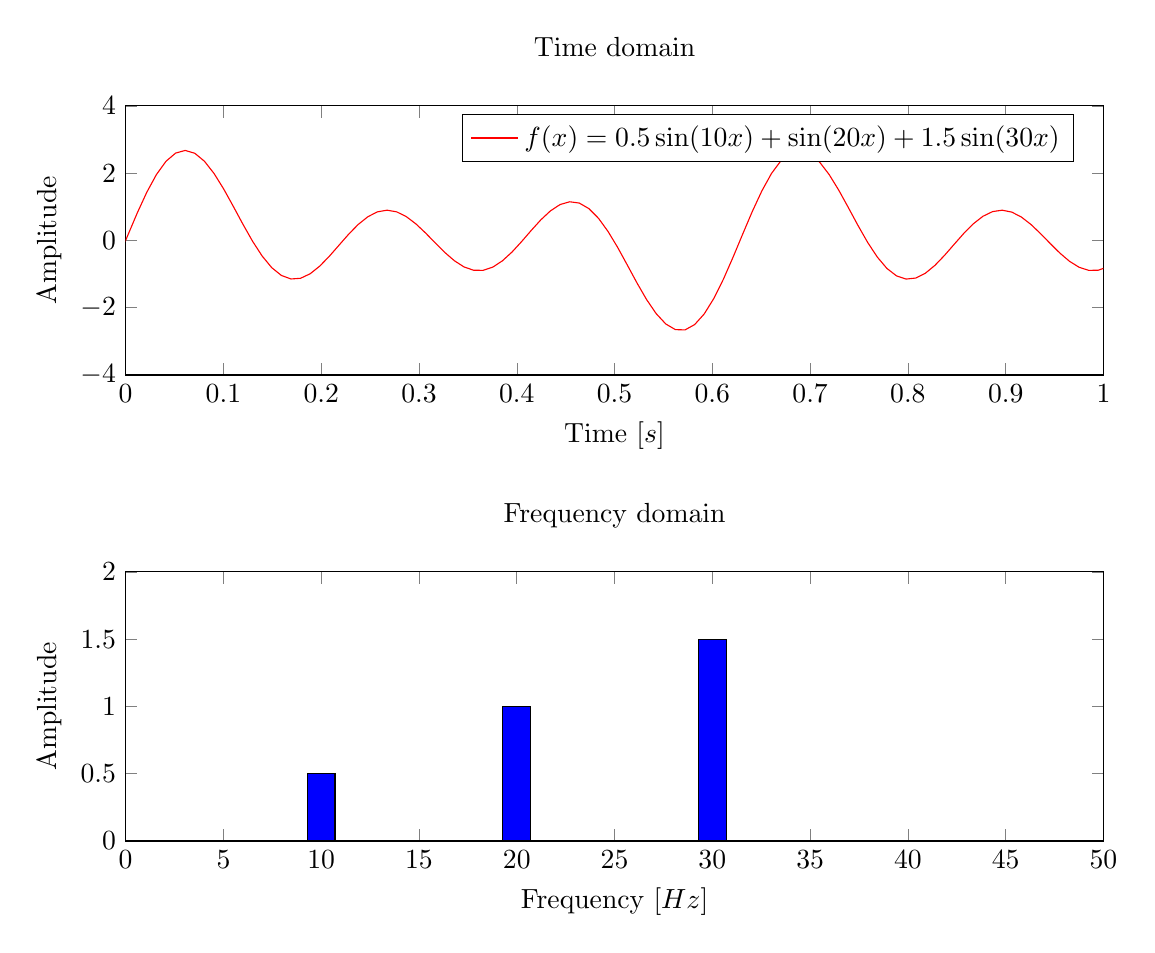
\begin{tikzpicture}
        \begin{groupplot}[group style={group name=my plots,group size= 1 by 2,horizontal sep =1.5cm,vertical sep =2cm},width=6cm]
            \nextgroupplot[
                legend pos=north east,
                trig format plots=rad,
                scaled ticks=false,
                tick label style={/pgf/number format/fixed},
                ymin=-4,
                ymax=4,
                xmin=0,
                xmax=1,
                ylabel={Amplitude},
                xlabel={Time $\left[s\right]$},
                width=14cm,
                height=5cm,
            ]
            \addlegendentry{$f(x) = 0.5\sin(10x) + \sin(20x) + 1.5\sin(30x)$}
            \addplot[domain=-0.5*pi:2*pi,samples=800,red] {0.5*sin(10*x) + sin(20*x) + 1.5*sin(30*x)};
            \nextgroupplot[
                legend pos=north east,
                trig format plots=rad,
                ymin=0,
                ymax=2.0,
                xmin=0,
                xmax=50,
                ylabel={Amplitude},
                xlabel={Frequency $\left[Hz\right]$},
                width=14cm,
                height=5cm,
                yshift=-0.5cm,
            ]
            \addplot[fill=blue,ybar] coordinates {
                    (10,0.5)
                    (20,1.0)
                    (30,1.5)
                };
            % \addplot[color=blue,mark=none] file {Data/frequencydomain.dat};
        \end{groupplot}
        \node[text width=12cm,align=center,anchor=north] at ([yshift=10mm]my plots c1r1.north) (cap1) {Time domain};
        \node[text width=12cm,align=center,anchor=north] at ([yshift=10mm]my plots c1r2.north) (cap2) {Frequency domain};
    \end{tikzpicture}
    \caption{Time domain and frequency domain of a signal}
    \label{fig:dft:ex1}
\end{figure}
\fi

Equation~\ref{eq:1} \cite[p.~92]{tan2013digital} describes the mathematical process of converting a signal $x$ to a spectrum $X$ of $x$ where $N$ is the number of samples, $n$ is the time step and $k$ is the frequency sample. When calculating $X\left(k\right) \forall\ k \in \left[0, N - 1\right]$ we clearly see that it will take $N^2$ multiplications. In 1965, Cooley and Tukey published a paper on an algorithm that could calculate the \gls{dft} in less than $2N\log(N)$ multiplications \cite{Cooley1964} called the Fast Fourier Transform (\gls{fft}).

\begin{align}
    X\left(k\right) = \sum\limits_{n=0}^{N-1}x\left(n\right)\cdot e^{-j\frac{2\pi}{N}kn},\ \ k = 0,1,2,\dots,N-1\label{eq:1}
\end{align}

\section{Fast Fourier Transform}
The Fast Fourier Transform algorithm composed by Cooley and Tukey is a recursive algorithm that runs in $O(N\log{}N)$ time. The following derivation is based on one found in this article from librow \cite{fft:derivation}. The notation for the imaginary number ($\sqrt{-1}$) was chosen to be $j$ instead of $i$ for consistency. If we expand the expression in Equation~\ref{eq:1}, presented in Chapter~\ref{ch:dft}, for $N = 8$ we get:

\begin{equation}
    X_{k} = x_0 + x_1e^{-j\frac{2\pi}{8}k} + x_2e^{-j\frac{2\pi}{8}2k} + x_3e^{-j\frac{2\pi}{8}3k} + x_4e^{-j\frac{2\pi}{8}4k} + x_5e^{-j\frac{2\pi}{8}5k} + x_6e^{-j\frac{2\pi}{8}6k} + x_7e^{-j\frac{2\pi}{8}7k}
\end{equation}\label{eq:first}

This expression can be factorized to use recurring factors of $e$ to:

\begin{equation}
\begin{aligned}
    X_{k} =&\ \ \ \ \ \ \ \ \ \ \ \ \left[x_0 + x_2e^{-j\frac{2\pi}{8}2k} + x_4e^{-j\frac{2\pi}{8}4k} + x_6e^{-j\frac{2\pi}{8}6k}\right]\\
           &+ e^{-j\frac{2\pi}{8}k}\left[x_1 + x_3e^{-j\frac{2\pi}{8}2k} + x_5e^{-j\frac{2\pi}{8}4k} + x_7e^{-j\frac{2\pi}{8}6k}\right]
\end{aligned}\label{eq:second}
\end{equation}

In turn, each bracket can be factorized to:

\begin{equation}
\begin{aligned}
    X_{k} =&\ \ \ \ \ \ \ \ \ \ \ \ \left[\left(x_0 + x_4e^{-j\frac{2\pi}{8}4k}\right) + e^{-j\frac{2\pi}{8}2k}\left(x_2 + x_6e^{-j\frac{2\pi}{8}4k}\right)\right]\\
           &+ e^{-j\frac{2\pi}{8}k}\left[\left(x_1 + x_5e^{-j\frac{2\pi}{8}4k}\right) + e^{-j\frac{2\pi}{8}2k}\left(x_3 + x_7e^{-j\frac{2\pi}{8}4k}\right)\right]
\end{aligned}\label{eq:third}
\end{equation}

And finally simplified to:

\begin{equation}
\begin{aligned}
    X_{k} =&\ \ \ \ \ \ \ \ \ \ \ \left[\left(x_0 + x_4e^{-j\pi k}\right) + e^{-j\frac{\pi}{2}k}\left(x_2 + x_6e^{-j\pi k}\right)\right]\\
           &+ e^{-j\frac{\pi}{4}k}\left[\left(x_1 + x_5e^{-j\pi k}\right) + e^{-j\frac{\pi}{2}k}\left(x_3 + x_7e^{-j\pi k}\right)\right]
\end{aligned}\label{eq:third:simplified}
\end{equation}

Because of symmetry around the unit circle we have the following rules:
\begin{gather*}
    e^{j(\phi + 2\pi)} = e^{j\phi}\\
    e^{j(\phi + \pi)} = -e^{j\phi}
\end{gather*}

We can use these rules to prove that the factor multiplied with the second term in each parenthesis in Equation~\ref{eq:third:simplified} will be 1 for $\{X_0, X_2, X_4, X_6\}$ and -1 for $\{X_1, X_3, X_5, X_7\}$. This means that each $e$-factor in front of the $x_n$ will be the same for all values of $k$. For the third level of the recursion (Equation~\ref{eq:third:simplified}), we have four parentheses with two factors for a total of eight operands.

The second level (Equation~\ref{eq:second}) have the same sums for $\{X_0, X_4\}$, $\{X_2, X_6\}$, $\{X_1, X_5\}$ and $\{X_3, X_7\}$.  They will have the factors $1$, $-1$, $-i$ and $i$ respectively. This level has two parentheses with four factors in each meaning that there is eight factors to sum here as for the third level. The first level (Equation~\ref{eq:first}) has eight unique factors to sum. In total, this recursion tree has $\log_2(8) = 3$ levels and each level has $8$ factors to sum. Generally this can be described as $\log_2(N)$ levels and $N$ factors at each level, giving a time complexity of $O(N\log{}N)$.

% http://www.librow.com/articles/article-10
% https://aaltodoc.aalto.fi/bitstream/handle/123456789/23201/master_Sugawara_Koki_2016.pdf?sequence=1

An iterative version of this algorithm would mimic the behaviour of the recursive version described previously. To demonstrate this process, the order of which the recursive implementation operates is visualized in Figure~\ref{fig:general:butterfly}. One butterfly operation is described in Figure~\ref{fig:butterfly:update}. With mathematical notation, this relation is described as $x'_a = x_a + x_b\omega^{k}_{N}$ and $x'_b = x_a - x_b\omega^{k}_{N}$, where $\omega^{k}_{N} = e^{-j\frac{2\pi}{N}}$. The first step would be to arrange the order in which the sample array $x$'s elements are in. One method for achieving this is to swap each element with the element at the bit-reverse of its index. Table~\ref{tab:rev:table} is a conversion table for an input array of size 8.

\ifrelease
\begin{figure}
    \centering
    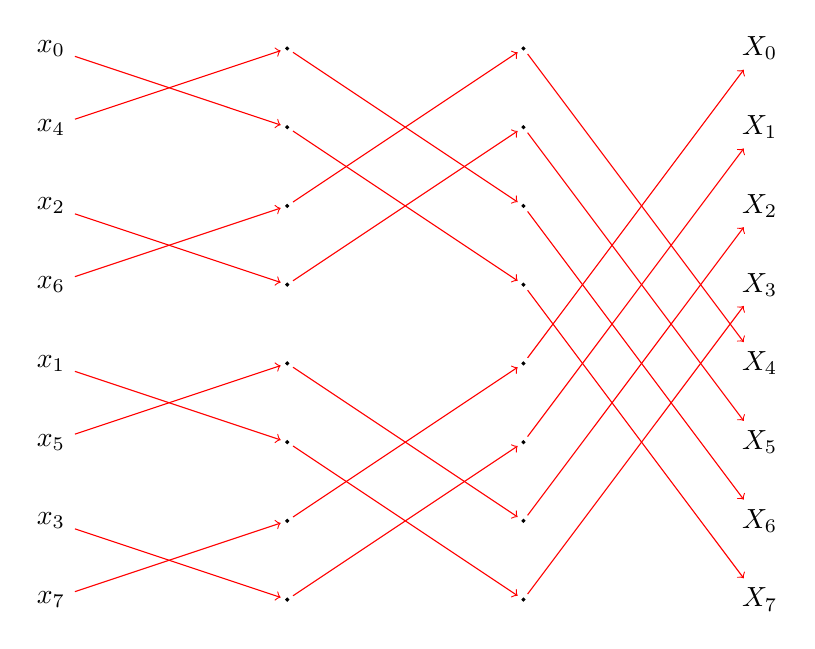
\begin{tikzpicture}[node distance=2cm]

        % nodes
        \node (f0) at (0, 7) {$x_0$};
        \node (f4) at (0, 6) {$x_4$};
        \node (f2) at (0, 5) {$x_2$};
        \node (f6) at (0, 4) {$x_6$};
        \node (f1) at (0, 3) {$x_1$};
        \node (f5) at (0, 2) {$x_5$};
        \node (f3) at (0, 1) {$x_3$};
        \node (f7) at (0, 0) {$x_7$};

        \node [draw,circle,fill=black,inner sep=0pt,outer sep=2pt] (h1) at (3, 7) {};
        \node [draw,circle,fill=black,inner sep=0pt,outer sep=2pt] (h2) at (3, 6) {};
        \node [draw,circle,fill=black,inner sep=0pt,outer sep=2pt] (h3) at (3, 5) {};
        \node [draw,circle,fill=black,inner sep=0pt,outer sep=2pt] (h4) at (3, 4) {};
        \node [draw,circle,fill=black,inner sep=0pt,outer sep=2pt] (h5) at (3, 3) {};
        \node [draw,circle,fill=black,inner sep=0pt,outer sep=2pt] (h6) at (3, 2) {};
        \node [draw,circle,fill=black,inner sep=0pt,outer sep=2pt] (h7) at (3, 1) {};
        \node [draw,circle,fill=black,inner sep=0pt,outer sep=2pt] (h8) at (3, 0) {};

        \node [draw,circle,fill=black,inner sep=0pt,outer sep=2pt] (2h1) at (6, 7) {};
        \node [draw,circle,fill=black,inner sep=0pt,outer sep=2pt] (2h2) at (6, 6) {};
        \node [draw,circle,fill=black,inner sep=0pt,outer sep=2pt] (2h3) at (6, 5) {};
        \node [draw,circle,fill=black,inner sep=0pt,outer sep=2pt] (2h4) at (6, 4) {};
        \node [draw,circle,fill=black,inner sep=0pt,outer sep=2pt] (2h5) at (6, 3) {};
        \node [draw,circle,fill=black,inner sep=0pt,outer sep=2pt] (2h6) at (6, 2) {};
        \node [draw,circle,fill=black,inner sep=0pt,outer sep=2pt] (2h7) at (6, 1) {};
        \node [draw,circle,fill=black,inner sep=0pt,outer sep=2pt] (2h8) at (6, 0) {};

        \node (3h1) at (9, 7) {$X_0$};
        \node (3h2) at (9, 6) {$X_1$};
        \node (3h3) at (9, 5) {$X_2$};
        \node (3h4) at (9, 4) {$X_3$};
        \node (3h5) at (9, 3) {$X_4$};
        \node (3h6) at (9, 2) {$X_5$};
        \node (3h7) at (9, 1) {$X_6$};
        \node (3h8) at (9, 0) {$X_7$};

        % arrows
        % First iteration
        \draw [->,draw=red] (f0) -- (h2);
        \draw [->,draw=red] (f4) -- (h1);
        \draw [->,draw=red] (f2) -- (h4);
        \draw [->,draw=red] (f6) -- (h3);
        \draw [->,draw=red] (f1) -- (h6);
        \draw [->,draw=red] (f5) -- (h5);
        \draw [->,draw=red] (f3) -- (h8);
        \draw [->,draw=red] (f7) -- (h7);

        % Second iteration
        \draw [->,draw=red] (h1) -- (2h3);
        \draw [->,draw=red] (h2) -- (2h4);
        \draw [->,draw=red] (h3) -- (2h1);
        \draw [->,draw=red] (h4) -- (2h2);
        \draw [->,draw=red] (h5) -- (2h7);
        \draw [->,draw=red] (h6) -- (2h8);
        \draw [->,draw=red] (h7) -- (2h5);
        \draw [->,draw=red] (h8) -- (2h6);

        % Third iteration
        \draw [->,draw=red] (2h1) -- (3h5);
        \draw [->,draw=red] (2h2) -- (3h6);
        \draw [->,draw=red] (2h3) -- (3h7);
        \draw [->,draw=red] (2h4) -- (3h8);
        \draw [->,draw=red] (2h5) -- (3h1);
        \draw [->,draw=red] (2h6) -- (3h2);
        \draw [->,draw=red] (2h7) -- (3h3);
        \draw [->,draw=red] (2h8) -- (3h4);
    \end{tikzpicture}
    \caption{Butterfly update for 8 values \cite{fft:derivation}}
    \label{fig:general:butterfly}
\end{figure}
\fi

\ifrelease
\begin{table}
    \centering
    \caption{Bit reversal conversion table for input size 8}
    \label{tab:rev:table}
    \begin{tabular}{|r|r||r|r|}
        \hline
        \textbf{normal dec} & \textbf{normal bin} & \textbf{reversed bin} & \textbf{reversed dec}\\
        \hline
        \texttt{0} & \texttt{000} & \texttt{000} & \texttt{0} \\
        \texttt{1} & \texttt{001} & \texttt{100} & \texttt{4} \\
        \texttt{2} & \texttt{010} & \texttt{010} & \texttt{2} \\
        \texttt{3} & \texttt{011} & \texttt{110} & \texttt{6} \\
        \texttt{4} & \texttt{100} & \texttt{001} & \texttt{1} \\
        \texttt{5} & \texttt{101} & \texttt{101} & \texttt{5} \\
        \texttt{6} & \texttt{110} & \texttt{011} & \texttt{3} \\
        \texttt{7} & \texttt{111} & \texttt{111} & \texttt{7} \\
        \hline
    \end{tabular}
\end{table}
\fi

\ifrelease
\begin{figure}
    \centering
    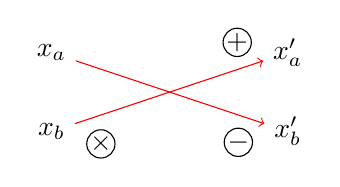
\begin{tikzpicture}[node distance=2cm]

        % nodes
        \node (A) at (0, 0) {$x_b$};
        \node (B) at (0, 1) {$x_a$};
        \node (C) at (3, 0) {$x'_b$};
        \node (D) at (3, 1) {$x'_a$};

        \node [draw,circle,above left=-3mm and 2mm of D,inner sep=0pt] (plus) {$+$};
        \node [draw,circle,below left=-3mm and 2mm of C,inner sep=0pt] (plus) {$-$};
        \node [draw,circle,below right=-2mm and 2mm of A,inner sep=0pt] (plus) {$\times$};

        % arrows
        \draw [->,draw=red] (A) -- (D);
        \draw [->,draw=red] (B) -- (C);

    \end{tikzpicture}
    \caption{Butterfly update \cite{fft:derivation}}
    \label{fig:butterfly:update}
\end{figure}
\fi

When we have achieved this, the operation order must be established. For the first iteration, the size of the gap between the operands is one. The next gap size is two and the third is four. It is now possible to construct an iterative algorithm. This process is shown in pseudocode in Algorithm~\ref{alg:fft}. The fist part of the algorithm is the Bit reversal. This has clearly $O(N)$ time complexity assuming the time complexity of bit\_reverse is bounded by the size of an integer. For the butterfly updates, the outer while loop will run for $\log{}N$ iterations and the two inner loops will run a total of $\frac{step}{2} \frac{N}{step} = \frac{N}{2}$ times. It is now clear that the time complexity of this algorithm is $O(N\log{}N)$.


\ifrelease
\begin{figure}[H]
    \begin{algorithm}[H]
        \KwData{Complex array $x = x_1, x_2, ..., x_N$ in time domain}
        \KwResult{Complex array $X = X_1, X_2, ..., X_N$ in frequency domain}

        \tcc{Bit reversal}
        \For{$i\gets 0$ \KwTo $N - 1$}{
            $r \gets$ bit\_reverse($i$)\\
            \If{$r > i$}{
                temp $\gets$ $x$[i]\\
                $x$[i] $\gets$ $x$[r]\\
                $x$[r] $\gets$ temp
            }
        }

        \tcc{Butterfly updates}
        $step \gets 2$\\
        \While{$step \leq N$}{
            \For{$k\gets 0$ \KwTo $step/2 - 1$}{
                \For{$p\gets 0$ \KwTo $N/step - 1$}{
                    $curr\gets p * step + k$\\
                    $x$[$curr$] $= x$[$curr$] $+$ $x$[$curr + step/2$]$*\omega^{k}_{step}$\\
                    $x$[$curr + step/2$] $= x$[$curr$] $-$ $x$[$curr + step/2$]$*\omega^{k}_{step}$
                }
            }
            $step \gets 2*step$
        }
        \textbf{return} $x$
        \caption{Iterative FFT}
        \label{alg:fft}
    \end{algorithm}
\end{figure}
\fi

\section{Related work}
A study called \emph{FFT benchmark on Android devices: Java versus JNI} \cite{Jr2013} was published in 2013 and investigated how two implementations of \gls{fft} performed on different Android devices. The main point of the study was to compare how a pure Java implementation would perform compared to a library written in C called \gls{fftw}. This library supports multi-threaded computation and this aspect is also covered in this study. Their benchmark application was run on 35 different devices with different versions to get a wide picture of how the algorithms ran on different phones.

\emph{Evaluating Performance of Android Platform Using Native C for Embedded Systems} \cite{Lee2010} explored how \gls{jni} overhead, arithmetic operations, memory access and heap allocation affected an application written in Java and native C. This study was written in 2010 when the Android \gls{ndk} was relatively new. Since then, many patches has been released, improving performance of code written in native C/C++. In this study, Dalvik VM was the virtual machine that executed the Dalvik bytecode. This study found that the \gls{jni} overhead was insignificant and took 0.15 ms to run in their testing environment. Their test results indicated that C was faster than Java in every case. The performance difference was largest in the memory access test and smallest in floating point calculations.

Published in 2016, \emph{Android App Energy Efficiency: The Impact of Language, Runtime, Compiler, and Implementation} \cite{Chen2016} presented a performance comparison between ART and native on Android. The main focus of the report was to find how much more efficient one of them were in terms of energy consumption. Their tests consisted of measuring battery drainage in power as well as execution time of different algorithms. It also compares performance differences between ART and Dalvik. The conclusion states that native performs much better than code running on the Dalvik VM. However, code compiled by ART improves greatly from Dalvik and performs almost the same as code compiled by Android \gls{ndk}.


\makechapter{Methodology}{Methodology\label{ch:methodology}}
\textit{To ensure that the experiment is carried out correctly, many different tools for measurements was evaluated. Different implementations of the FFT are also compared to choose the ones that would typically be used in an Android project.}
% Test how large the cost of JNI
% Debug/VMDebug libraries

% Preparation
% What tools are used? Phone, software, libraries (currenttimemillis vs nantotime etc),
% Different thread pools
% Measure execution time
% Measure memory consumption
% Benchmark Environment (Which phone, Android version, Compiler version, Java version, compiler flags)
% Benchmark Environment parameters (Started apps, memory left, started processes? cpu throttling by mobile case?)
% Profilers for time and memory measurement
% Disable Instant Run??
% Which operations should be included?
% Should I Measure every operation in detail?
% Garbage collection discussion (You cannot control it)
\section{Experiment model}

% http://lessthanoptimal.github.io/Java-Matrix-Benchmark/manual/MethodologyRuntimeBenchmark/
% In java, we cannot control GC, which can lead to varying results
% In java, do not use string concatenation (will ask for memory)
% Measure first, optimize later

\subsection{Hardware}
\subsection{Benchmark Environment}
\subsection{Time measurement}
\subsection{Memory measurement}

% How will the results be represented?
% How will I interpret the results
% How many times will the programs be executed
% Statistical significance
% What is included in the calculation, what is not (adding result to string etc)
\section{Evaluation}

\subsection{Data representation}
\subsection{Data interpretation}
\subsection{Statistical significance}

% Description of which algorithms that are available, which one that is used and why
% Detailed description/comparison between the code.
% Correctness test/verification??
% Complexity
% Test data: sizes of data, datatypes (long vs int vs float vs double)
\section{Fast Fourier Transform Algorithms}

\subsection{Java libraries}
JTransforms\cite{jtransforms:benchmark}

\subsection{C++ libraries}
\cite{FFTW05}



\makechapter{Experiments}{Experiments\label{ch:experiments}}
% TODO: Rename as Result?
\textit{Summarizing the chapter}



\makechapter{Discussion}{Discussion\label{ch:discussion}}
\textit{The discussion chapter covers how the JNI affects performance, how efficient smaller FFT libraries are, why the optimization gave the results found in Chapter~\ref{ch:results} - Results and the efficiency difference between floats and doubles.}

\section{JNI Overhead}
The test results from the JNI tests showed that the overhead is small relative to the computation of the FFT algorithm. As long as it is being run once per calculation, it will not affect the performance significantly. If the JNI is called in a loop when it might not be necessary, the overhead can add up and become a larger part of the total execution time. Another thing to note is that the execution time stay within about 10 \textmu s.

The confidence intervals overlap for many of the values, meaning we cannot say whether one input yields a faster execution time than the other. Some larger block sizes has lower execution time than smaller block sizes and some grow for larger input. It is then reasonable to assume that nothing is done to the arrays when they are passed to the JNI, only pointers are copied. The \texttt{GetPrimitiveArrayCritical} and \texttt{ReleasePrimitiveArrayCritical} seem to introduce overhead when used on larger arrays. % <= CITE THIS ... as described in

Regarding the spike in mean for some JNI results, this can be a cause of one large execution time skewing the results. This is actually the case for the \textbf{Convert} tests with block size 1024 as seen in Figure~\ref{fig:raw:jni:convert:1024} found in Appendix B. A reason for this could be that the garbage collector began executing during the timing of the test.

\section{Simplicity and Efficiency}

The slowest algorithm was the Java Princeton Recursive. The reason for this is because it executes many method calls. For each method call, registers must be saved by pushing them onto a stack, function arguments must them be moved to appropriate registers and a jump instruction to the new code must be executed. When the function has finished executing, the registers are popped from the stack. This causes a lot of overhead.

Additionally, each call creates new \texttt{Complex} arrays when splitting up the array in odd and even indices. Lastly, when combining the arrays, new \texttt{Complex} objects are created each time an operation is done between two complex numbers. The reason for the is because the \texttt{Complex} class creates immutable objects. This slows down the process and increases memory consumption, increasing work for the garbage collector.

The C++ version of the Princeton Recursive algorithm is faster than the Java version. One big difference is that the \texttt{std::complex} type used in C++ does not create new instances each time is is being operated with. Instead, they are placed on the stack. This lowers the number of calls requesting more memory from the heap. Depending on the situation for the program, there is a risk that the program must ask the system for more memory, slowing down the allocation process.

Additionally, this will increase the work for the garbage collector, increasing the risk of it being triggered during the tests. To prevent the number of allocations you are doing inside a repeated process you commonly reuse allocated memory. This is done by pre-allocating the necessary arrays or other data structures and overwrite the results for each call. Avoiding calls to the \texttt{new} keyword in a method that is called multiple times can increase time and memory efficiency.

Of the algorithms tested in the FFT library tests, KISS FFT was the fastest. It is more optimized than the \enquote{basic} implementations found in the Columbia and Princeton algorithms. In C++, Princeton Iterative and Columbia Iterative were the fastest and in Java, Columbia Iterative was the fastest. The reason for Princeton Iterative being faster in C++ is, as for Java Princeton Recursive, because it uses the \texttt{Complex} class to represent complex numbers. Because Java Columbia Iterative used double arrays to represent real and imaginary numbers, no new objects needed to be created.

The results from Chapter~\ref{ch:gc} - Garbage Collection show that the Java Princeton algorithms caused the GC to run. This behaviour was as expected because they called new during their execution. Java Columbia did not cause any garbage collection and neither did any of the C++ algorithms.

One thing that is clear is that the Columbia Iterative algorithm is the best one to choose from of the Java versions. It performs better than both Princeton Iterative and Princeton Recursive. It also allows simple modifications such as changing between using \texttt{float}s or  \texttt{double}s to represent the data.

% The reason Princeton Iterative and Princeton Recursive is slower in Java than in C++ is because they operate with \texttt{Complex} elements. Each time two \texttt{Complex} numbers are added, multiplied or subtracted, a new \texttt{Complex} object is created.

As we have seen in the tests, choosing an iterative implementation is preferable and choosing the correctly implemented iterative implementation is also important. It is possible to compare implementations by setting up small tests. This is a small time investment that ensures that you get the performance you need in a program. It is also possible to read through the implementation, looking for places where it allocates memory and edit it so that it uses an already allocated array. This reduces the number of calls for more memory which lessens the chance of a garbage collect.

Comparing the Java and C++ implementations of the Columbia Iterative FFT, for \emph{small}-\emph{large} block sizes, the Java version is almost as fast as the C++ version. For the block sizes added in the \emph{extra large} group, the C++ version perform better. If you were to choose between the C++ and the Java variant of Columbia, it is better to choose the Java version if the performance requirement allows it. Avoiding having to implement a JNI bridge between Java and native is more preferable than the small increase in performance.

Another argument why it is sensible to choose the Java version is that is has enough performance for processing to allow graphical rendering in 60 \gls{fps}. Let's say we have an application that visualizes sound with a sampling frequency of 44100 Hz and updates the screen at 60 frames per second. It has 16.66 ms to do all the processing needed between the screen updates. If we want to have double precision numbers and use Java it is possible to do an FFT with a size of \textbf{32768}.

% => More common to use sliding window, minimize latency <=

This size is more than needed and would require $32768/44100\approx 743 $ ms to sample. The fastest Java algorithm for double point precision ran in $12$ ms for this block size. As we can see, in relation, the time it takes to execute an FFT is only a small fraction of the time it takes to gather the same number of samples. This is important because it allows larger FFT sizes from the sampled audio, increasing the frequency resolution in the results, while still being sufficiently fast.

For smaller block sizes (\emph{medium} and \emph{large}), common when sampling low frequencies such as speech and acceleration data, it is relevant to have fast transforming for these sizes. Comparing C++ and Java we see that Java is not that much slower, at best, than C++. This gives an incentive to use Java, allowing more consistent code and does not add the complexity of JNI.

When the block sizes are large, a bigger difference is found between the algorithms. One reason for this is the impact the garbage collection has when triggered during the timing of an algorithm. The pauses can range between, depending on the work done in the garbage collect, 0.468-23.760 ms.

KISS FFT was the fastest of all the native implementations. This was because of the optimizations done to improve its performance. Using multiple radix implementations of the FFT, it is possible to get more performance at the cost of higher code complexity. It shows the potential in doing small optimizations that does not rely on multi-core or other architecture dependent optimization techniques.

How memory is used differs between algorithms. As seen in Chapter~\ref{ch:gc}, only four tests caused the garbage collector to be run. Java Princeton Iterative and Recursive with both \texttt{float} and \texttt{double} as primary data types were the algorithms causing this. This is because they create new arrays each time they are called. The garbage collector needed to remove each array that was allocated each call, thus increasing the total work the garbage collector must achieve.

\section{Vectorization as Optimization}

As the results show, vectorization was an improvement in regards to efficiency. This was as expected because it is possible to process more elements for each instruction. The optimizations implicitly implemented loop unrolling because more operations were covered in the body of the loop, resulting in less jump instructions, leading to less instructions in total.

The Recursive NEON implementation did not perform much worse than the Iterative version. The difference between the implementations were of a smaller factor than between Princeton Iterative and Recursive. One reason for this could be that because the twiddle factors are moved so that they are closer in cache in a two dimensional array for the recursive version. They are placed in order of access to reduce the number of cache misses. This could be the reason for the performance increase.

% IMPRTNT => MORE PROS?? <= IMPRTNT 

One disadvantage of using NEON intrinsics is the fact that you cannot run it on all CPU architectures. Not all Android devices runs on ARM, and not all ARMv7 supports NEON \cite{arm:neon}. This makes it less compatible if the program depends on its optimizations. One example of an optimization that is architecture independent and works on all multi-core CPUs is parallelization. Another disadvantage of NEON is that it makes a program harder to maintain. It introduces complexity to the program in addition to JNI. 

A possible implementation could be optimized by fitting all the components in cache. This reduces the overhead of fetching data from memory which would slow down the overall performance. If it is not possible for the data to fit in cache, you can rewrite the algorithm such that the elements are stored close by in order of access. This will result in less cache invalidation and less direct memory reads.

When needing to do a lot of processing with the data in frequency domain, a fast FFT will help in lowering the total execution time. If the data is also transformed back into time domain, for example when you want to filter out noise in an audio signal and play it back. Another reason you would want a fast FFT is when the computation time for some validation need to be as fast as possible. An example of this is voice recognition where we want answers in reasonable time. Another example could be to do image recognition on fingerprints for fast biometric authentication.

\section{Floats and Doubles}
One reason for using the \texttt{float} data type is that they are stored as 32-bit values instead of 64-bit values as \texttt{double}s are stored. This means that the program requires less memory and reduces the risk of triggering the \texttt{GC\_FOR\_ALLOC} due to the lack of free memory distributed to the process. Most modern devices has pipelined floating point operations to optimize calculations \cite{android:float}. In the case of the experiments performed in this thesis, \texttt{float} performed better than \texttt{double} for the device used in the tests.

The reason for this is that because \texttt{float}s are half the size of \texttt{double}s, they have a large chance of fitting in cache. Depending on the cache size, it could be beneficial to use the \texttt{float} data type. This is an important point to keep in mind. A reason why you would not use \texttt{float}s is when you need the precision of \texttt{double}s or when the performance difference is not an issue or non-existent.

The test results showed that there is a big difference when computing floats and doubles for in both Java and C++. It is also the case that some \texttt{float} tests in Java execute at half the execution time of the corresponding algorithm for \texttt{double} in C++. This shows the importance, on some architectures with different cache sizes, to choose the appropriate data structures as they can impact the performance greatly.


\makechapter{Conclusion}{Conclusion\label{ch:conclusion}}
\textit{Describing text}

\hilight{When choosing a java version, choose Columbia Iterative (Conclusion)}

\hilight{Native is architecture dependent. Not always the possible to use it}


\appendix

\makeappendix{Appendix A}{Example appendix}

Converted code, raw data and the benchmark program used for the tests can be found in the following repository:

\begin{center}
    \url{https://github.com/anddani/thesis}
\end{center}



% \lstinputlisting[
%     language=Java,
%     basicstyle=\scriptsize,
%     label={lst:complex},
%     caption={Complex.java \cite{princeton:complex}},
% ]{BenchmarkApp/app/src/main/java/com/example/algo/benchmarkapp/algorithms/Complex.java}
%
% \lstinputlisting[
%     language=C++,
%     basicstyle=\scriptsize,
%     label={lst:recursive:neon},
%     caption={Conversion of a recursive SSE FFT \cite{neon:recursive:details}},
% ]{BenchmarkApp/app/src/main/cpp/FFTRecursiveNeon.cpp}
%
% \lstinputlisting[
%     language=C++,
%     basicstyle=\scriptsize,
%     label={lst:iterative:neon},
%     caption={Conversion of an iterative SSE FFT \cite{manyears:code}},
% ]{BenchmarkApp/app/src/main/cpp/FFTIterativeNeon.cpp}
%
% \lstinputlisting[
%     language=C++,
%     basicstyle=\scriptsize,
%     label={lst:iterative:columbia},
%     caption={Conversion of Columbia Iterative \cite{columbia:iterative}},
% ]{BenchmarkApp/app/src/main/cpp/FFTColumbiaConverted.cpp}
%
% \lstinputlisting[
%     language=C++,
%     basicstyle=\scriptsize,
%     label={lst:iterative:princeton},
%     caption={Conversion of Princeton Iterative and Recursive \cite{princeton:recursive,princeton:iterative}},
% ]{BenchmarkApp/app/src/main/cpp/FFTPrincetonConverted.cpp}


%%==================================================================
%% BIBLIOGRAPHY
%%==================================================================
\bibliographystyle{ieeetr}

\fancyhead[LO]{}%
\fancyhead[RE]{}%
\fancyhead[LE]{\thepage}%
\fancyhead[RO]{\thepage}

\bibliography{references}

\end{document}
